% !TEX encoding = UTF-8 Unicode
\documentclass[a4paper]{article}

\usepackage{color}
\usepackage{url}
\usepackage[T2A]{fontenc}
\usepackage[utf8]{inputenc}
\usepackage{graphicx}

\usepackage[english,serbian]{babel}

\usepackage[unicode]{hyperref}
\hypersetup{colorlinks,citecolor=green,filecolor=green,linkcolor=blue,urlcolor=blue}

\usepackage{listings}

\newtheorem{primer}{Primer}[section]

\definecolor{mygreen}{rgb}{0,0.6,0}
\definecolor{mygray}{rgb}{0.5,0.5,0.5}
\definecolor{mymauve}{rgb}{0.58,0,0.82}

\lstset{ 
  backgroundcolor=\color{white},
  basicstyle=\scriptsize\ttfamily,
  breakatwhitespace=false,
  breaklines=true,
  captionpos=b,
  commentstyle=\color{mygreen},
  deletekeywords={...},            
  escapeinside={\%*}{*)},          
  extendedchars=true,
  firstnumber=1000,              
  frame=single,	                
  keepspaces=true,
  keywordstyle=\color{blue},     
  language=Python,                
  morekeywords={*,...},
  numbers=left, 
  numbersep=5pt,                  
  numberstyle=\tiny\color{mygray}, 
  rulecolor=\color{black},
  showspaces=false,
  showstringspaces=false,
  showtabs=false,
  stepnumber=2, 
  stringstyle=\color{mymauve},
  tabsize=2,
  title=\lstname
}

\begin{document}

\title{Programski jezik F\#\\ \small{Seminarski rad u okviru kursa\\Metodologija stručnog i naučnog rada\\ Matematički fakultet}}

\author{Tijana Todorov, Tamara Garibović,\\ David Nedeljković, Mihajlo Vićentijević \\ tijana.todorov710@gmail.com, t.garibovic1995@gmail.com, \\ dnedeljkovic710@gmail.com, mihajlovicent@gmail.com}

%\date{9.~april 2015.}

\maketitle

\abstract{
Dodati na kraju sazetak.}

\tableofcontents

\newpage

\section{Uvod}
\label{sec:uvod}

Dodati na kraju uvod u temu i obavezno izmeniti trenutni radni naslov.

\section{Poreklo programskog jezika F\#}
\label{sec:poreklo}

U 2018. godini F\# opisan je u dokumentaciji kao "funkcionalni programski jezik koji se pokreće na .NET platformi" \cite{early_history}, ali odakle je on potekao?

Istorija programskog jezika F\# datira još od 1970. godine pa sve do danas. U ranim 70-im godinama na Univerzitetu u Edinburgu Robin Milner sa još nekoliko svojih kolega razvija jezik ML (Meta-Language) baziran na programskom jeziku LISP. Njegova onsnovna namena bila je pragmatičnog karaktera. Osmišljen je da pomogne u dokazivanju LCF (Logical computable functions) \cite{Milner:1972:LCF:891954} teorema. ML jezik je koren svih jezika koji pripadaju familiji strogo tipiziranih funkcionalnih jezika, kao npr: Miranda, Haskell, Standard ML, Ocaml, EdinburghML, ReasonML, PureScript, a među njima i F\#.

Sve do danas ključne ideje ove familije jezika ostaju osnova jezika F\# koji se nadogradjivao kasnije iz dana u dan. 

Tokom 80-ih godina dolazi do velike ekspanzije u kompjuterskoj industriji. Kako su se brzo razvijali softverski alati tako su se takođe pojavljivali novi jezici i programske paradigme. U tom periodu i Microsoft doživljava veliku ekspanziju kao kompanija koja razvija operativne sisteme i aplikacije. Međutim, u ovom periodu, a najviše u kasnim 80-im godinama pojavljuje se novi, objektno-orjentisani talas razmišljanja u programiranju koji veoma utiče na razvoj softvera.

Početkom 90-ih godina, dok je Microsoft težio da održi monopol na tržištu i dok je u fokusu i dalje bila objektno-orjentisana paradigma, strogo tipizirani funkcionalni jezici bili su manje aktivni i okrenuti su ka razvitku na drugim poljima. Njihova primena uglavnom je imala ulogu u pronalaženju bagova, održavanju sistema i verifikaciji hardvera i softvera. Primeri jezika koji su se koristili za izgradnju ovakvih sistema su: Edinburgh ML, Standard ML, Ocaml, Caml Light, LISP. Takođe, neki funkcionalni jezci razvijeni su u cilju istraživanja u okviru paralelnog programiranja, kao što su Parallel ML i vrsta paralelnog Haskell-a \cite{early_history}. 

\subsection{Zašto je nastao jezik F\#?}
\label{subsec:nastanak}

Tokom 90-ih godina Microsoft razvija .NET \cite{microsoft_.net,early_history} platformu za razvoj softvera. Ideja je bila da se omogući međusobna kompatibilnost više programskih jezika, odnosno da svaki jezik podržan na ovoj platformi može da koristi kôd nekog drugog jezika platforme. Glavni cilj Microsoft-a bio je da se na ovoj platformi podrži što veći broj jezika iz različitih paradigmi. 

U okviru ovoga Don Syme razija projekat SML.NET koji je za ideju imao preusmeravanje Standard ML-a na .NET. Sistem je imao visok kvalitet, ali nije bio usvojen od strane programera. Početkom 2000-ih platforma .NET je već uveliko zaživela, ali za jezik SML.NET nije bilo većeg interesovanja. Autor je imao veliku želju da implementira strogo tipiziran funkcionalni jezik na način koji bi zainteresovao veliki broj programera. U razmatranje ulazi i jezik OCaml, ali prethodno dolazi do pokušaja implementacije Haskell-a za .NET. Ovaj pokušaj bio je samo delimično uspešan i primenjen na malim programima. Rad na daljoj implementaciji je zaustavljen.

U decembru 2001. godine Don Syme u razmatranje vraća jezik OCaml i razvija projekat Caml.NET koji će se kasnije preimenovati u F\#.

Inicijalna ideja F\# programskog jezika bila je jednostavna. Trebalo je da poveže prednosti OCaml programskog jezika sa prednostima .NET platforme. 2002. godine pojavljuje se prva verzija F\# 0.5 koja bila je slabo primećena. Don Syme 2004. godine nastavlja intenzivno da razvija ovaj jezik, a početkom 2005. godine izbacuje prvu potpunu verziju F\#-a \cite{early_history}.
Poslednja aktuelna verzija jezika je F\# 4.1 \cite{fsharp}.

\subsection{Koji programski jezici su najviše uticali na razvoj jezika F$\#$?}
\label{subsec:uticaj}

Najveći značaj za razvoj jezika F\# imaju jezik SML (Standard ML) i CAML (Categorical Abstarct Machine Language) porodica jezika koja je razvijana na Nacionalnom institutu za istraživanje informatike i automatizacije u Francuskoj 1994. godine \cite{Harrop:2008:FS:1481410}. U okviru ovog projekta pod nazivom “Cristal project” razvija se jezik Objective Caml koji ima veoma visoke performanse i naučnici ga koriste na Linux i MAC OS X platformama. Kao što je već ranije opisano, jezik OCaml i .NET platforma imali su najveći uticaj na razvoj jezika F\#. Na slici \ref{fig:stablo} može se videti deo razvojnog stabla koji ovo prikazuje.

\begin{figure}[h!]
\begin{center}
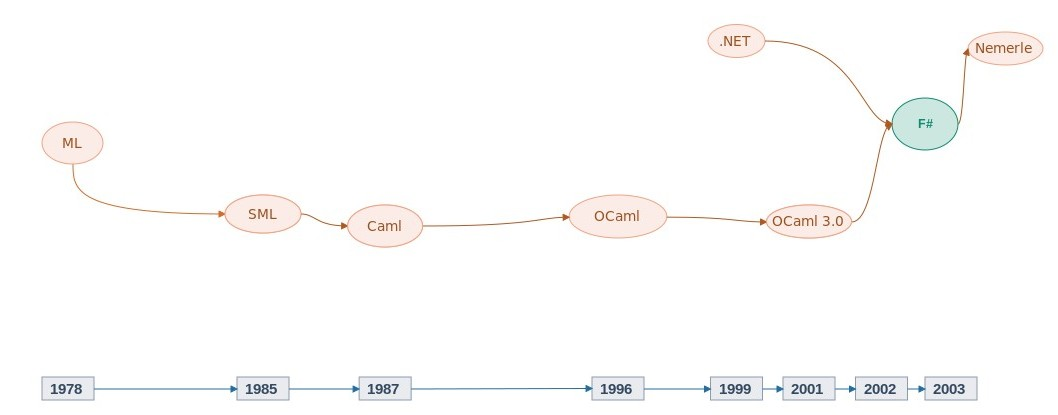
\includegraphics[scale=0.29]{stablo.jpg}
\end{center}
\caption{Razvojno stablo}
\label{fig:stablo}
\end{figure}


\section{Primena i mogućnosti}
\label{sec:primena}

Snaga F\# programskog jezika leži u svedenoj sintaksi koja omogućava laku čitljivost kôda, kao i efikasan razvoj programa koji zahtevaju primenu složenih matematičkih algoritama. Jezik omogućava brzo generisanje prototipova i njihovu brzu transformaciju u produkcioni kôd. Kôd napisan u F\#-u lako se može paralelizovati, što je posebno značajno danas kada svi novi računari imaju više jezgara. F\# danas ima široku primenu u obradi baza podataka, finansijskog modelovanja, statistici i bioinformatici. Takodje, domen primene svakodnevno raste.

F\# je jezik koji ima pretežno funkcionalne karakteristike, ali on je svoju primenu pronašao u još mnogo vrsta programiranja. Neki od njih su: imperativno, objektno-orjentisano, paralelno, distribuirano, asinhrono, meta programiranje, veb programiranje, skript programiranje, analitičko programiranje, i sl. Danas se on može koristiti na velikom broju sistema, kao što su: Linux, MAC, Windows, Android, iOS, i sl. O ovome će biti više reči u nastavku. 


\section{Osnovne osobine programskog jezika F\#}

Neke od osnovnih osobina programskog jezika F\# su:\\

	- \textbf{Bezbedan}: F\# programi se temeljno proveravaju pre izvršenja, što ga čini bezbednim za pokretanje.

	- \textbf{Funkcionalan}: Funkcije mogu biti ugnježdene, prosleđene kao argumenti drugim funkcijama i vraćene kao povratna vrednost.

	- \textbf{Strogo tipiziran}: Provera tipova se vrši u toku kompilacije, kako bi se utvrdilo da su dobro definisani. 

	- \textbf{Automatski zaključuje tipove}: Tipovi vrednosti se automatski zaključuju prilikom kompilacije u zavisnosti od konteksta u kome se javljaju, što dovodi do toga da se eksplicitno navođenje retko dešava.

	- \textbf{Kompatibilan}: F\# programi mogu da pozivaju i da budu pozvani iz drugih programa koji su napisani na nekom od jezika koje podržava .NET platforma, kao na primer C\#\cite{microsoft_c}. 
\\
%Nešto više o njima\cite{Harrop:2008:FS:1481410}.
 
	Još neke specifičnosti jezika: \\
	
	- Za razliku od drugih programskih jezika struktura \textbf{if/elif/else} u svakoj grani ima povratnu vrednost.
	 
	- Povratna vrednost ne mora uvek biti vraćena ključnom reči return. Ukoliko je \textbf{return} izostavljen, kao povratna vrednost se uzima poslednja izvršena naredba.
	 
	- Korišćenjem ključne reči \textbf{let} definišemo promenljive koje se ne mogu menjati što kod čini sigurnijim od slučajnih promena. Ukoliko smo sigurni da će se vrednost promenljive menjati, uz let se dodaje ključna reč \textbf{mutable}.
	 
	- Struktura \textbf{switch/case} je u F\# zamenjena pattern matching-om\cite{expertFS}.
	 
	- Pored uobičajenih tipova podataka podržanih u većini programskih jezika, F\# podržava novi tip \textbf{option type}, koji označava vrednost promenljive koja može da postoji a i ne mora. Dve moguće vrednosti ovog tipa su: Some(x) i None.

\section{Funkcionalno programiranje}

%dodati naucni rad o ovoj oblasti


Kao glavna, funkcionalna paradigma programskog jezika F\# podržava osnovne koncepte koji su podržani i od strane nekih drugih programskih jezika. U ovom odeljku nećemo davati prevelik značaj osnovama funkcionalne paradigme, već ćemo akcenat staviti na \textbf{pattern matching}\cite{expertFS}.\\

Jedan od važnih mehanizama u F\# programiranju jeste pattern matching. Pattern matching se predstavlja kao match ... with ... konstrukcija koja kombinuje mehanizme dekompozicije i kontrole toka za poklapanje obrazaca. Kao takav, možemo ga koristiti sa  jednostavnim kolekcijama(list,tuple) i option vrednostima. Naredni listing \ref{primer} pokazuje kako se definiše pattern matching.
\\
\begin{lstlisting}[caption={Primer pattern matching-a\cite{expertFS}},frame=single, label=primer]
let urlFilter url agent =
 match (url,agent) with
 | "http://www.control.org", 99 -> true
 | "http://www.kaos.org" , _ -> false
 | _, 86 -> true
 | _ -> false
\end{lstlisting} 

Izvedeni tip funkcije je:

\begin{lstlisting}
val urlFilter: string -> int -> bool
\end{lstlisting}

Izraz nakon ključne reči match je tupple tipa(string * int). Svako pravilo obrasca se uvodi sa simbolom | iza koga sledi pravilo. Nakon navodjenja pravila sledi simbol -> nakon čega sledi rezultat. Kada se izvrše, pravila obrasca se koriste jedan po jedan i prvi obrazac koji je poklopljen određuje rezultat. Prvi obrazac se poklapa ukoliko su navedene identične vrednosti, dok poslednja tri, na mestima gde se javlja simbol $\_$ za ulazne parametre mogu da imaju bilo koju vrednost. U tabeli \ref{tab:tabela1} prikazaćemo koje vrste obrazaca postoje u F\# i na koji način ih možemo formirati.
 
\begin{table}[h!]
\begin{center}
\caption{Načini formiranja obrazaca u F\#}
\begin{tabular}{|c|c|c|} \hline
Opšti oblik& Vrsta& Primer\\ \hline
(pat, ... ,pat) &Tuple pattern&(1,2,("3",x))
\\ \hline
[pat, ... ,pat] &List pattern&[x;y;z]\\ \hline
[|pat, ... ,pat|] &Array pattern&['a';'b';'c']\\ \hline
null &Null test pattern&null\\ \hline
\end{tabular}
\label{tab:tabela1}
\end{center}
\end{table}


\section{Asinhrono i paralelno programiranje}

Razlog zbog kojeg izučavamo asinhrono i paralelno programiranje se ogleda u maksimalnoj iskorišćenosti hardvera. Ranije se ovaj način programiranja izbegavao zbog dodatne složenosti i rizika od bagova. Sa pojavom velikog broja biblioteka u kombinaciji sa funkcionalnim programiranjem i izbegavanjem bočnih efekata ovaj problem je smanjen. Fokus ćemo staviti na to kako ubrzati računanje u F\# koristeći asinhrono i paralelno programiranje. Izvršavanje koda se odvija pomoću niti i F\# biblioteka. 
Iskoristite prednosti više procesora i jezgara tako sto cete podeliti jedan posao na vise manjih. Najvažniji razlog uvođenja ova dva načina programiranja je ubrzanje izvršavanja koda.


\subsection{Asinhrono programiranje} 

Opisuje programe i operacije koje se izvršavaju u pozadini i završavaju nakon nekog vremena (primer: preuzimanje novog email-a bez čestog proveravanja). Asinhroni programi na .NET platformi su pisani korišćenjem modela asinhronog programiranja (APM). APM je obrazac koji deli asinhrone operacije na dve metode: BeginOperation i EndOperation. Kada se pozove BeginOperation operacije počinju sa asinhronim izvršavanjem koje po završetku pozivaju EndOperation koji dohvata rezultat asinhronog izračunavanja. Problemi koji nastaju korišćenjem ovog obrasca su: 

	- izostavljanje poziva EndOperation dolazi do neželjenih efekata, curenja memorije 
 
	- ukoliko se nekoliko asinhronih izračunavanja vrati nazad teško je pratiti tok programa
	
	- posledica prethodnog problema uzrokuje pojavu špageti programiranja

Umesto APM-a sve asinhrone operacije ćemo izvršavati pomoću F\# biblioteke asinhronih radnih tokova\cite{workFlow}. Ključna reč async se koristi za kreiranje bloka u koji se smešta kod za izvršavanje, korišćenjem let! i do! operatora. Rezultat ovog izvršavanja će biti tipa Async<T>\cite{theAL}.

\subsection{Paralelno programiranje}

Paralelno programiranje se koristi za podelu poslova na n delova kako bi se dobilo n puta brže izvršavanje što je retko u praksi. Najjednostavniji način koriščćenja paralelnog programiranja na .NET 4.0 platformi se zasniva na upotrebi Parallel Extesions biblioteke(PFX)\cite{progFsPFX}. Jedna od pogodnosti PFX biblioteke je ta što programer ne mora da misli o kontroli rada niti. Za razliku od paralelnog, asinhroni tok izvršavanja je dostupan i na prethodnim verzijama .NET platforme. Task objekat predstavlja osnovnu strukturu PFX paralelizma, koji ima zadatak da izvrši posao nakon nekog vremena. Kao takav, nije dovoljan za paralelne aplikacije. Zbog problema koji se javlja pri radu Task objekta sa deljivim podacima uvodi se zaključavanje podatka(exclusive lock). PFX biblioteka uvodi nove tipove kolekcija System.Collections.Concurrent \cite{sysCC} kao rešenje prethodnog problema.  


\section{Radni okviri}

Najpoznatiji i najznačajniji radni okvir(framework) za ovaj programski jezik je .NET koji je ranije već pomeut. Ovaj radni okvir je potpuno besplatan i na njemu je moguće kreirati veliki broj različitih aplikacija. On podržava veliki broj programskih jezika iz različitih paradigmi, editora i biblioteka za igradnju mobilnih i veb aplikacija. 

Temelj .NET platforme je zajednička jezička infrastruktura CLI (Common Language Infrastructure). Pokretanje F\# koda na ovoj platformi se vrši tako što na samom početku kompajler prevodi kod u binarni fajl koji je preveden na asemblerski jezik višeg nivoa koji se zove MSIL (Microsoft Intermediate Language). Implementacija na CLI kompajleru ovog asemblerskog koda u toku izvršavanja je mnogo brža nego da je kod samo interpretiran i ova kompilacija se izvršava u trenutku\cite{progFs}.
Kod koji je preveden u MSIL i izvršen u trenutku, predstavlja kod za upravljanje za razliku od kodova pisanih na progamskim jezicima kao što su C ili C++ koji su sirovi kodovi.   

Postoje neke prednosti za prolazak kroz CLI ili upravljani kod a ne direktnog kompiliranja na mašinski nivo:	

	- kompatibilnost medju jezicima
	
	- mogućnost rada na više platformi
	
	- mašinska nezavisnost
\\

.NET platforma ima jos jednu prednost a to je prikupljanje smeća sto omogućava programeru da ne razmislja mnogo o alociranju memorije i oslobadjanju, već da se samo skoncentriše na pisanje koda. Iako ne mora da obraća pažnju na smeće i rad sa memorijom poželjno je da programer zna na koji način taj sakupljač smeća radi, kako on oslobadja memoriju i rešava taj problem.

Naravno da ova platforma nije jedina koja se koristi za ovaj progamski jezik, pored nje postoje: web radni okviri (Suave, Fable, ASP.NET Core, Giraffe, WebSharper, Freya, NancyFx, Serving Requests with IHttpHandler, Serving Requests with Azure, Functions, Pure F\# Web API 2.0, SignalR, ServiceStack, ASP.NET Blazor) i radni okviri za testiranje weba (Web Testing, Frameworks, Canopy for Client-side Testing, Unit Testing Libraries)\cite{fwFs}.

\section{Uputstvo za instalaciju}

U ovom poglavlju biće opisano uputstvo za instalaciju programskog jezika F\# na Windows i Linux operativnim sistemima.

\subsection{Uputstvo za Windows}

Na ovom operativnom sistemu postoje tri načina za instalaciju F\#-a. To su: Visual studio\cite{vStud}, Visual Studio Code \cite{vStudCode} i JetBrains Rider \cite{jetBrains}.

\subsubsection{Visual studio}
	
Na Windows operativnim sistemima se uglavnom koristi Visual Studio alat. Visual studio 2017 je alat koji dolazi sa podrškom za F\# u svim verzijama: Professional, Enterprise i Community (verzija je potpuno besplatna). Međutim, ukoliko imate  već instaliran Visual Studio 2012/13/15  Professional ili above možete ga takođe koristiti zato što i on podržava alate za F\# iako nije toliko napredan kao Visual Studio 2017.

\subsubsection{Visual Studio Code}
	
Visual Studio Code je besplatna platforma koja podržava mnogo jezika,a među njima i F\# . On je podržan od strane Ionide\cite{ionide}.

\textbf{1.korak:} Instalirati Visual studio Code za Windows

\textbf{2.korak:} Pritisnuti \textbf{Ctrl+Shift+p} i ukucati sledeću naredbu za instalaciju Ionide paketa za Visual Strudio Code:
\\
\begin{lstlisting}
 ext install Ionide-fsharp
\end{lstlisting}
 
\subsubsection{JetBrains Rider}

JetBrains Rider je platforma .NET IDE izgrađena je pomoću InteliJ i  ReSharper tehnologije. JetBrains nudi podršku .NET i .NET Core aplikacijama na svim platformama.

\textbf{1.korak:} Instalirati JetBrains za Windows

\textbf{2.korak}(opciono): instalirati poslednju .NED Core SDK

Takođe vam je potrebno da instalirate ceo Visual Studio ili F\# kompajler.


\subsection{Uputstvo za Linux}

Instalacija F\# na Linuxu se izvršava na potpuno identičan način za Ubuntu, Mint i Debian verziju.

\subsubsection{Ubuntu/Mint/Debian}

\textbf{1.korak:} Dodajte Mono\cite{mono} repozitorijum vašem menadžeru paketa.

\textbf{2.korak:} Instalirati F\# koji će istovremeno povući novu verziju Mono-a ukoliko je to potrebno.
\\
\begin{lstlisting}
sudo apt-get update
sudo apt-get install fsharp
\end{lstlisting}
 

\section{Zaključak}
\label{sec:zakljucak}

Sta je zakljucak celog rada.

\addcontentsline{toc}{section}{Literatura}
\appendix
\bibliography{seminarski} 
\bibliographystyle{plain}


\end{document}